\documentclass[10pt]{amsart}
\usepackage[margin=1.4in]{geometry}
\usepackage{amssymb,amsmath,enumitem,url}
\usepackage{graphicx,subfig}
\graphicspath{ {./visualizations/} }

\newcommand{\D}{\mathrm{d}}
\newcommand{\I}{\mathrm{i}}
\DeclareMathOperator{\E}{e}
\DeclareMathOperator{\OO}{O}
\DeclareMathOperator{\oo}{o}
\DeclareMathOperator{\erfc}{erfc}
\DeclareMathOperator{\real}{Re}
\DeclareMathOperator{\imag}{Im}
\usepackage{tikz}
\usepackage[framemethod=tikz]{mdframed}
\theoremstyle{nonumberplain}

\mdtheorem[innertopmargin=-5pt]{sol}{Solution}
%\newmdtheoremenv[innertopmargin=-5pt]{sol}{Solution}

\begin{document}
\pagestyle{empty}

\newcommand{\mline}{\vspace{.2in}\hrule\vspace{.2in}}

\noindent
\text{Hunter Lybbert} \\
\text{Student ID: 2426454} \\
\text{03-31-25} \\
\text{HMS 581:}
\text{Infectious Disease Modeling} \\
% header containing your name, student number, due date, course, and the homework number as a title.

\title{\bf {Quiz} }


\maketitle
\noindent
Solutions to the problems which are described in the entrance quiz to \textit{HMS 581}.
\mline
\begin{enumerate}[label={\bf {Question \arabic*}}]
\item (Linear Algebra): \\
\begin{enumerate}

\item Dominant Eigenvector and corresponding eigenvalue of
$$A =
\begin{bmatrix}
0.5 & 0.25 \\
0.5 & -0.125
\end{bmatrix}
$$

\textit{Solution:} \\
Solving using the characteristic equation gives us the following
\begin{align*}
(0.5 - \lambda)(-0.125-\lambda) - 0.5(0.25) &= 0 \\
\lambda^2 -0.5\lambda + 0.125\lambda + 0.5(-0.125) - 0.5(0.25) &= 0 \\
\lambda^2 -0.375\lambda -0.0625 - 0.125 &= 0 \\
\lambda^2 -0.375\lambda -0.1875 &= 0 \\
\implies \lambda = \frac{0.375 \pm \sqrt{(-0.375)^2 - 4(-0.1875)}}{2} &.
\end{align*}
I have verified this with the results from calculating it with NumPy in Python.
The dominant eigenvector is the eigenvector corresponding to the eigenvalue which is largest in absolute value.
In our case the larger eigenvalue in absolute value is 
$\lambda = 0.65936465$ with the eigenvector
$$
v_1 = \begin{bmatrix}
0.84324302 \\
0.53753252
\end{bmatrix}.
$$

\item If $x = [1 \;\: 1]^T$, let $y = Ax$. Further let $|\cdot|_2$ denote the $l^2$ norm or Euclidean distance. Without doing the calculation which will be larger $|x|_2$ or $|y|_2$? Why? \\

\textit{Solution:} \\
I believe $|x|_2$ will be larger.
If my linear algebra memory is serving me correctly the dominant eigenvalue being less than 1 would imply that the linear transformation which the matrix $A$ represents is compressing input vectors that it is operating on.
Therefore, the resultant $|y|_2$ would be smaller since $A$ is compressing input vectors. \\

\item Let $\hat x$ and $\hat y$ denote the normalized vectors.
We calculated $| \hat x - v_1|$ and $|\hat y - v_1|$.

\textit{Solution:} \\
I might have been able to guess that the second quantity is smaller since the matrix $A$ is compressing values and they are getting closer to the dominant eigenvalue.

\end{enumerate}
\qed \\
\newpage

\item (ODE Question): \\
\begin{enumerate}
\item Solve the following differential equation:
$$\frac{dy}{dx} = ry, \quad \text{ with } y(0) = y_0.$$

\textit{Solution:}\\
We begin by using separation of variables 
\begin{align*}
\frac{dy}{dx} &= ry \\
\frac 1 y dy &= rdx \\
\int \frac 1 y dy &= \int rdx \\
\log y &= rx + C \\
y(x) &= \E^{rx}\E^{C}.
\end{align*}
Now let's utilize our initial condition $y(0) = y_0$ to determine the constant $\E^C$.
\begin{align*}
y(0) &= \E^{r0}\E^C \\
y_0 &= \E^{0}\E^C \\
y_0 &= \E^C.
\end{align*}
Therefore our solution given this initial condition is
$$
y(x) = y_0\E^{rx}.
$$

\item Solve the following differential equation:
$$
\frac{dy}{dx} = ry\left(1 - \frac y K\right) \quad \text{ with } y(0) = y_0
$$

\textit{Solution:} \\
Similarly let's use separation of variables
\begin{align*}
\frac{dy}{dx} &= ry\left(1 - \frac y K\right) \\
\frac 1 {y - \frac{y^2} K}dy &= rdx \\
\int \frac 1 {y - \frac{y^2} K}dy &= \int rdx \\
\int - \frac 1 {y^2} \frac 1 {\frac 1 K - \frac 1 y}dy &= \int rdx
\end{align*}
Consider using a $u$ sub at this point.
Perhaps let $u = \frac 1 K - \frac 1 y$ then $du = \frac 1 {y^2}$.
plugging this in we now have
\begin{align*}
\int - \frac 1 {u}du &= \int rdx \\
- \log u &= rx + C \\
\log \left( \frac 1 K - \frac 1 y \right) &= - rx + C \\
\frac 1 K - \frac 1 y &= \E^{- rx}C \\
- \frac 1 y &= \E^{- rx}C + \frac 1K \\
y(x) &= \frac 1 {- \E^{- rx}C - \frac 1K}.
\end{align*}
Our initial condition gives us
\begin{align*}
y(0) &= \frac 1 {- \E^{- r0}C - \frac 1K} \\
y_0 &= \frac 1 {-C - \frac 1K} \\
- \frac 1 {y_0} - \frac 1 K &= C.
\end{align*}
Finally, we have
$$
y(x) = \frac 1 {- \E^{- rx}\left( - \frac 1 {y_0} - \frac 1 K \right) - \frac 1K}.
$$

\item For the second equation, assuming $r > 0$ and $K > 0$, identify all the equilibrium and assess their stability. \\

\textit{Solution:} \\
Let $\dot y = \frac {dy}{dx}$, the equilibrium occur where $\dot y = 0$ that is
\begin{align*}
\frac {dy}{dx} &= ry\left(1 - \frac y K\right) \\
\dot y &= ry\left(1 - \frac y K\right) \\
0 &= ry\left(1 - \frac y K\right)
\end{align*}
Which occurs when $y^* = 0, K$.
I will use Linear Stability Analysis (LSA) to determine the stability of these fixed points (or equilibrium).
Let's additionally let $f(y) = ry\left(1 - y/K\right)$.
Then using LSA we want to determine if $f^\prime(y^*)$ is greater than or less than 0 for each fixed point, $y^*$.
Since we have $f^\prime(y) = r - 2ry/K$, then
\begin{align*}
f^\prime(0) &= r > 0 \implies \text{the fixed point at 0 is unstable} \\
f^\prime(K) &= -r < 0 \implies \text{the fixed point at K is stable}
\end{align*}
\end{enumerate}
\qed \\
\newpage

\item (Coding Question...with probability): \\
Suppose you are playing a betting game where you:
\begin{enumerate}
\item Start with $\$X$
\item Each round of the game costs \$1
\item For each round, you flip a coin whose chance of heads coming up is $p \in (0, 1)$
\item If the coin lands heads, you win the round and receive \$2 (your original \$1 back and an additional \$1 for winning).
If the coin lands tails, you lose the round, and receive \$0.
\item You repeat playing rounds of the game, betting and flipping the coin until you either run out of money (i.e., you lose the game) or you reach $\$Y$ (and then you stop, i.e., you win the game).
For sanity purposes, also assume you stop the game after 1,000 rounds even if you haven’t lost all your money or hit $\$Y$ :) \\
\end{enumerate}
Let us refer to a series of rounds where you start at $\$X$ and either end with \$0 or $\$Y$ as a “game”.
Write code that will simulate “a game” $n$ times, randomly ‘flipping’ a coin for every round of every game, and store the amount of money you have throughout the rounds for each game (as well as the final outcome).

\begin{enumerate}
\item Run the game $n = 1,000$ times with $X = 5$, $p = 0.5$, and $Y = 10$. Plot a histogram of the number of rounds needed to finish the game.
Plot the trajectories of money held by round by game (with round as the x-axis and money held as the $y$-axis.

\begin{figure}[h]
	\centering
	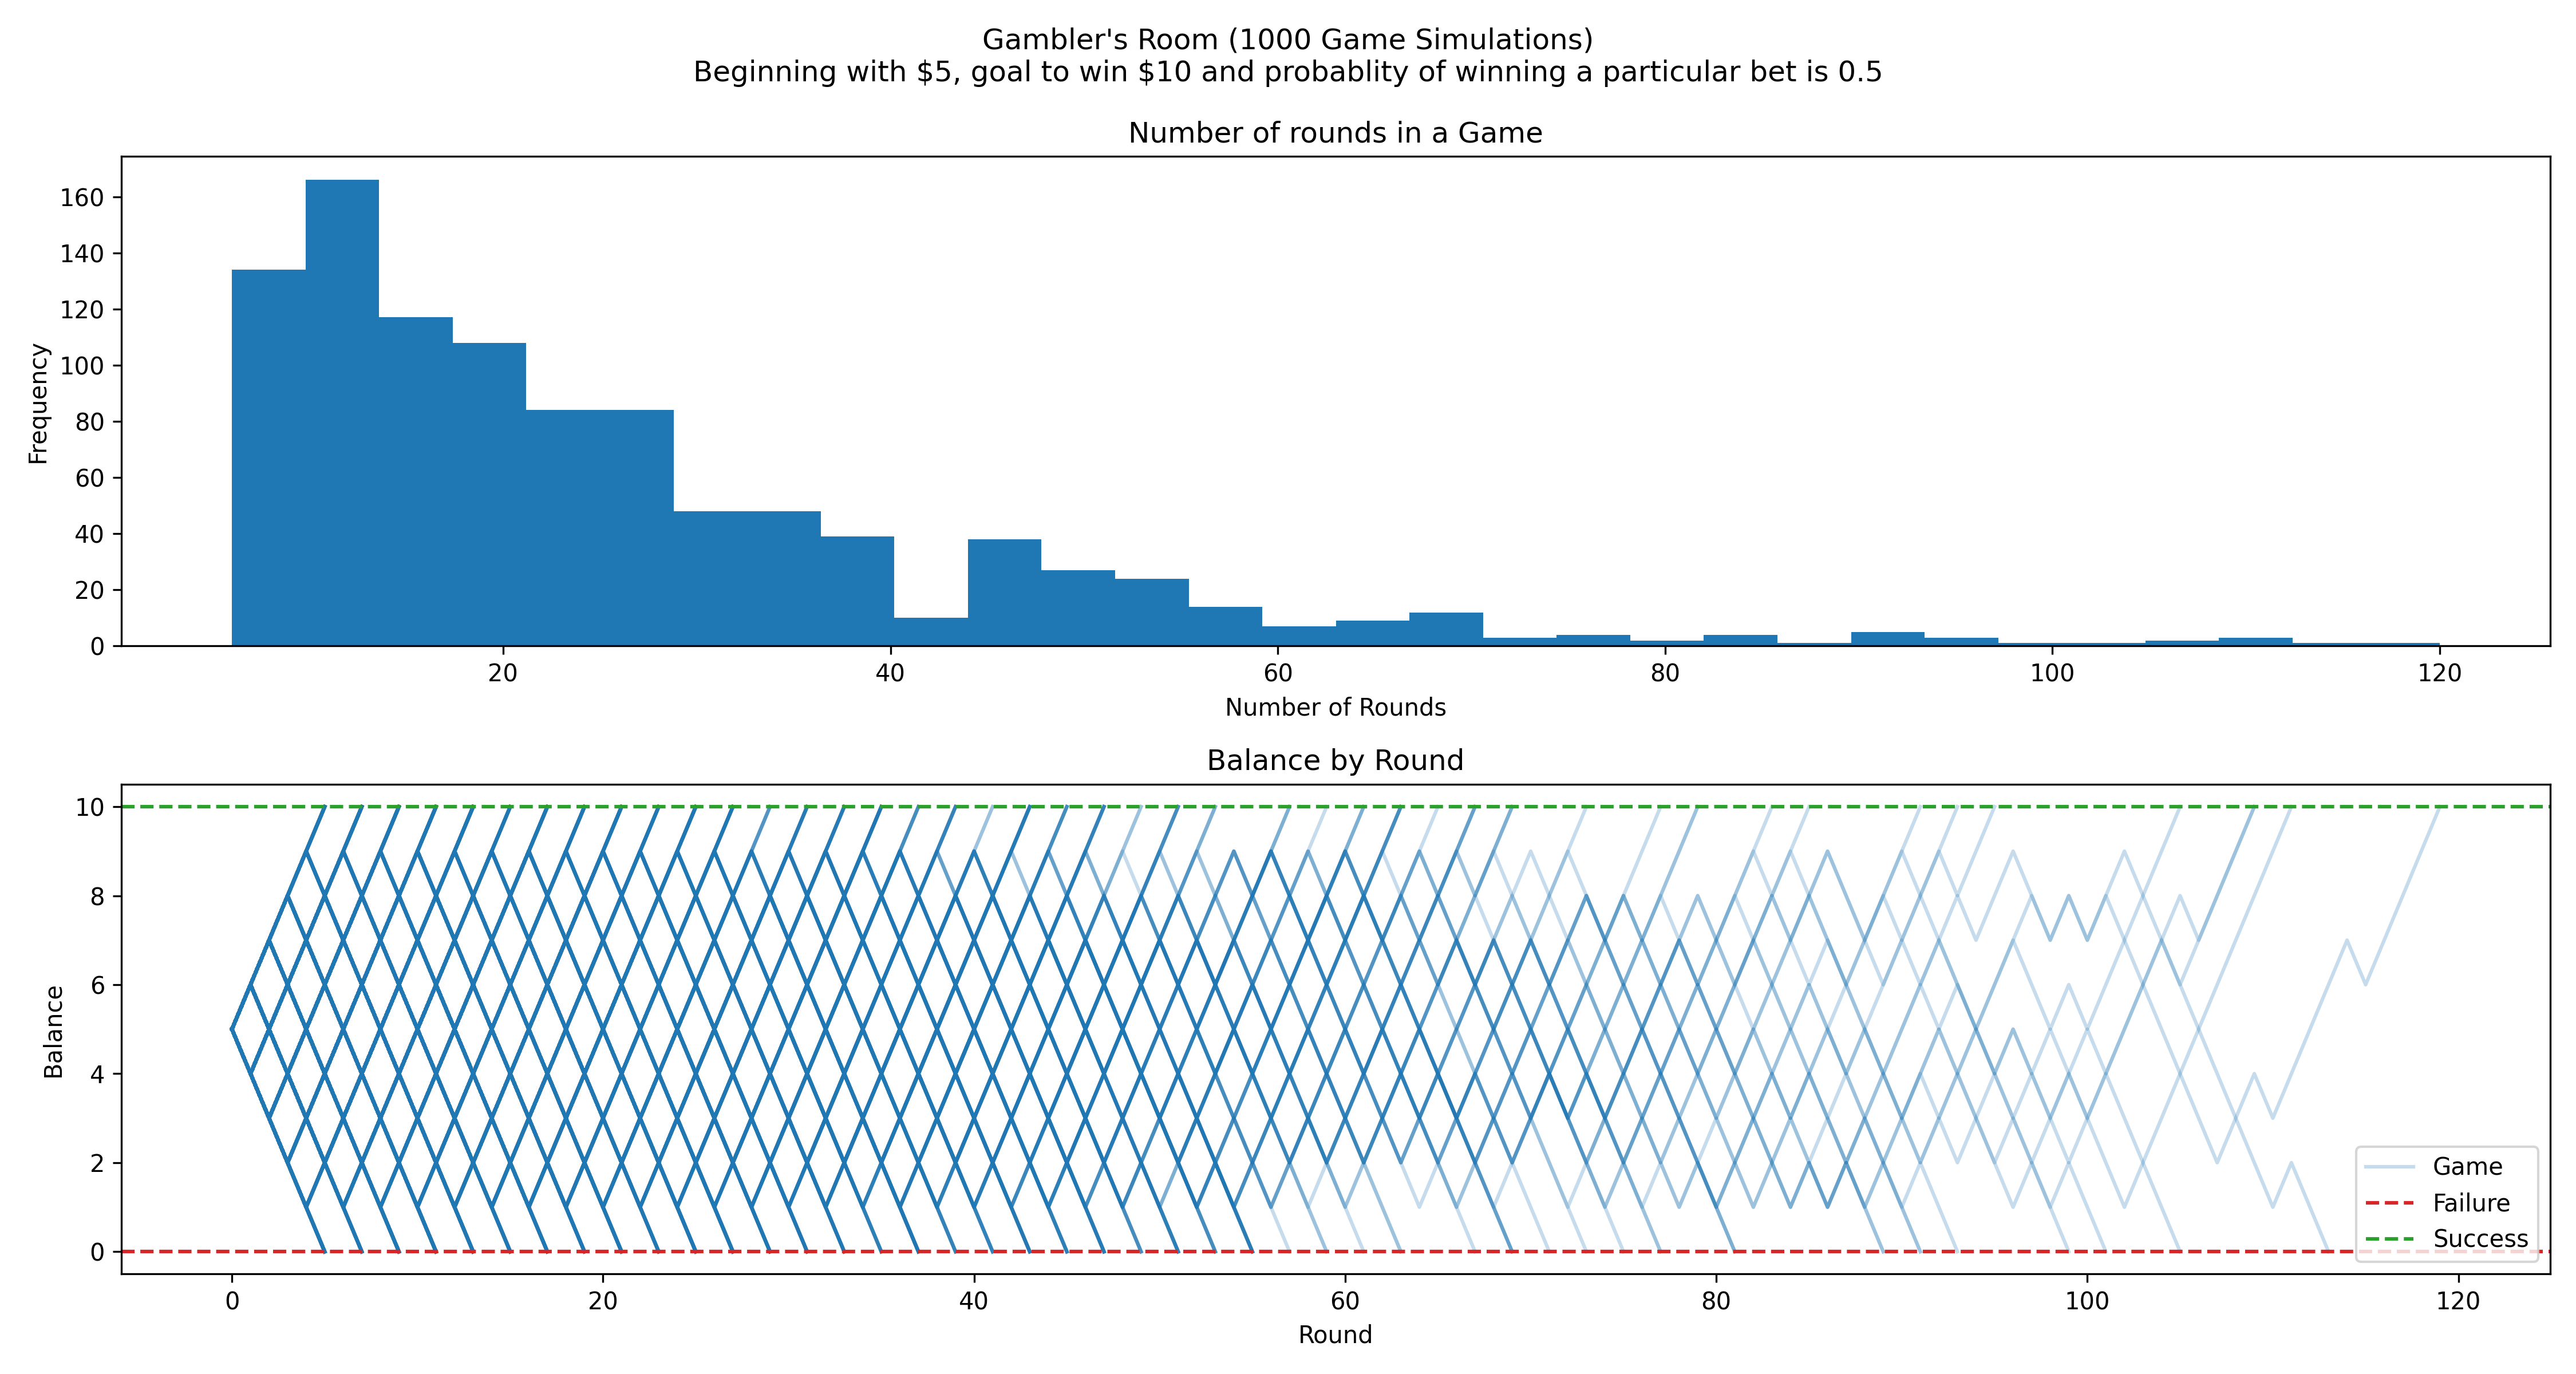
\includegraphics[width=1\textwidth]{balance_by_round_and_histogram.png}
 	\caption{These are the histogram and balances over time for 1000 simulations run starting with \$5 and trying to achieve \$10.
	and where the probability of winning a particular bet, $p = 0.5$.}\label{fig:f1}
\end{figure}

\item Run the game $n = 100$ times with $X = 10$ and $Y = 20$ for $p = 0.05, 0.1, 0.15, . . . 0.9, 0.95$.
For each value of $p$ track the fraction of the games that ends with \$0.
Plot the values of $p$ on the $x$-axis and fraction of games lost.
\item Repeat (b) for $Y = 30, 40, \text{ and } 50$ and plot the resulting output on the same plot as (b), indicating which output comes from which value of $Y$.
\begin{figure}[h]
	\centering
	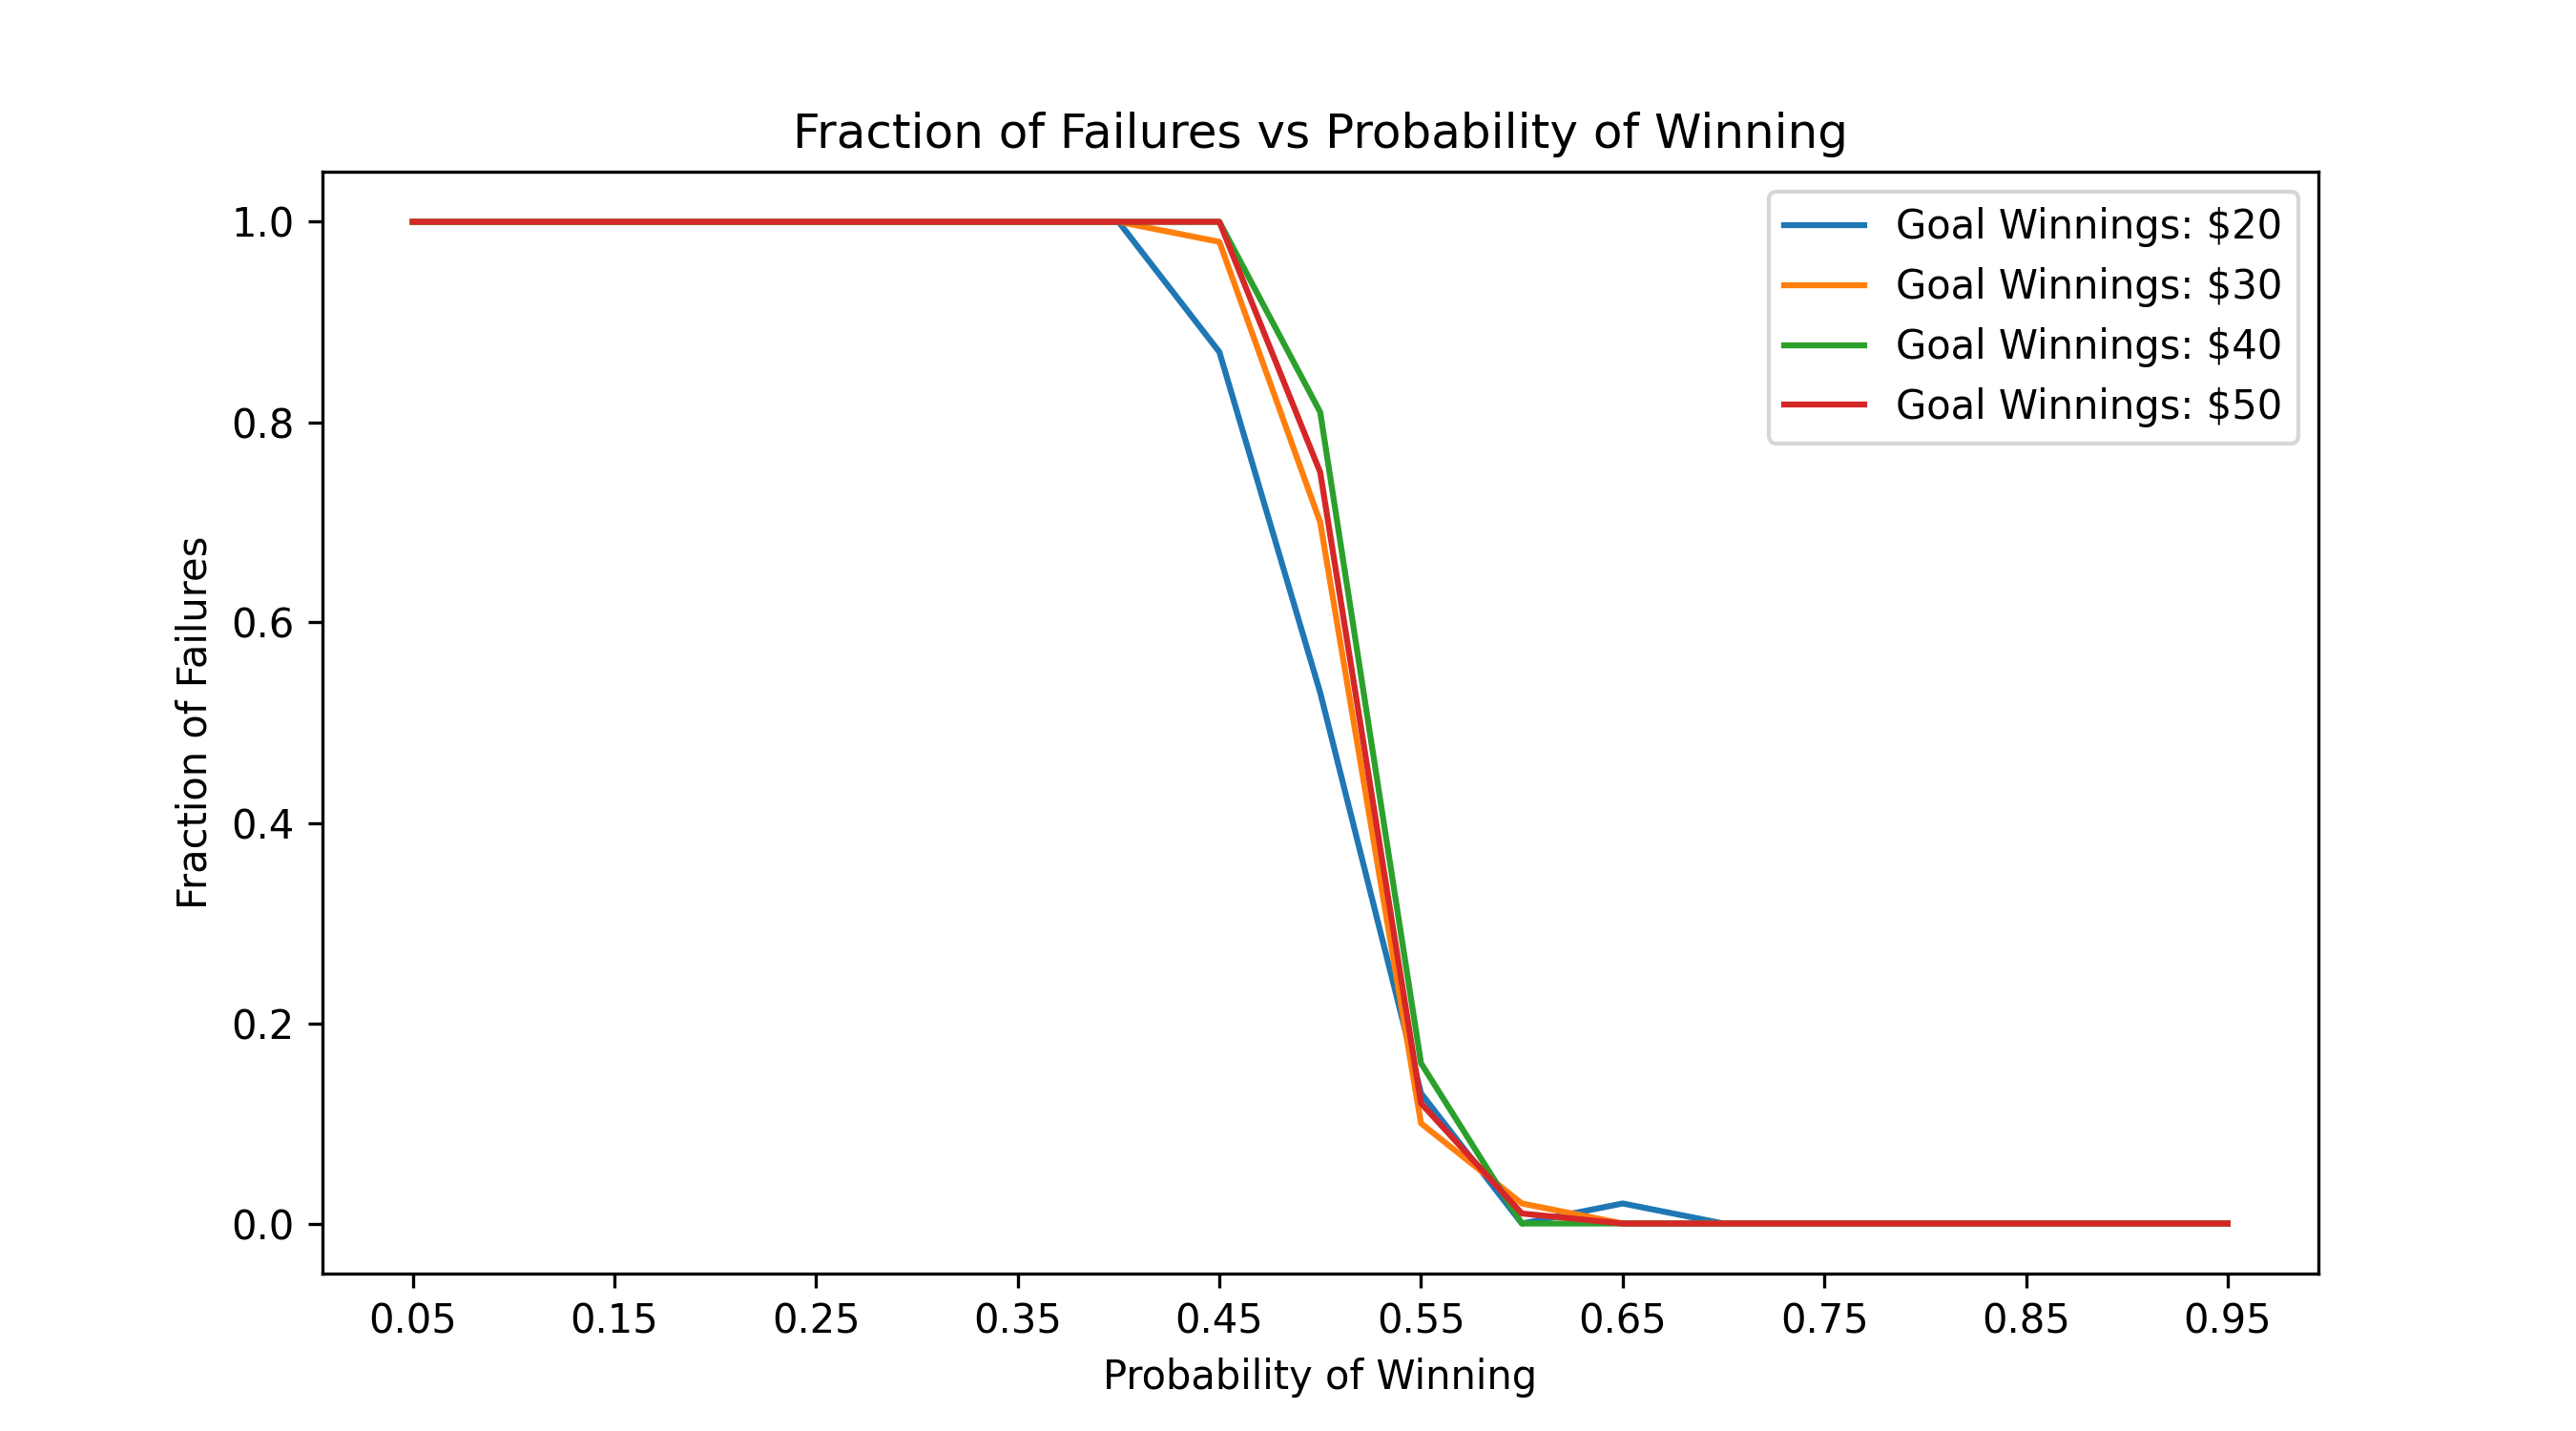
\includegraphics[width=1\textwidth]{fraction_of_failures_vs_probability.png}
 	\caption{The fraction of failed games for each goal winnings value.
	Notice, that while the probability is low 100\% of the trials failed.
	However, as the probability of success increases the fraction of failures rapidly disappears.
	}\label{fig:f2}
\end{figure}
\end{enumerate}
\qed \\
\newpage

\item (Epidemiology question):
\begin{enumerate}
\item Define Incidence and prevalence with respect to Covid-19. \\
\textit{Solution:}
Incidence is the rate at which new cases occur over a specific space and time.
Not sure how to adapt this to be more covid specific, but I will come back to it if I have time.
\textbf{TODO: Utilize this resource I think: https://pubmed.ncbi.nlm.nih.gov/35279023/}
While prevalence is the proportion of a population that has a specific disease or health condition at a particular point in time.

\item Define Infection and case with respect to Covid-19. \\
\textit{Solution:}
Infection refers to people are infected with Covid-19, regardless of whether they show symptoms or have been tested,
Infections can include both symptomatic and asymptomatic cases.
Next, cases are confirmed and identified through testing.


\item Can the mortality rate ever be larger than 1? Can a case fatality rate ever be larger than 1? \\
\textit{Solution:}
\textbf{TODO: Come back if time.}

\item Give an example of a pathogen system were an individual can only become infected once. More than once (other than COVID). \\
\textit{Solution:}
\textbf{TODO: Come back if time.}

\item Give one example each of a pathogen transmission system that is (a) direct, (b) indirect, (c) vector-bourne. \\
\textit{Solution:}
\textbf{TODO: Come back if time.}
\qed \\

\end{enumerate}

\end{enumerate}

\end{document}

%%% Local Variables:
%%% mode: latex
%%% TeX-master: t
%%% End:
